\documentclass[aspectratio=169,10pt,t]{beamer}
\usetheme{faeder}

\usepackage{pgfplots}
\pgfplotsset{compat=1.18}
\usepackage{hyperref}
\usepackage{qrcode}
\hypersetup{colorlinks=true,urlcolor=fsTeal,linkcolor=fsNavy}

% Pathway cartoon for the cytokine-STAT-SOCS example.
%   \roadmap{k}      highlight step k, fade later steps
%   \roadmap{99}     show every step normally
% Optional first argument is passed to tikzpicture, e.g. \roadmap[scale=0.8]{3}.
\tikzset{
  fsactive/.style={draw=fsAccent,line width=1.4pt,text=fsAccent},
  fsfuture/.style={opacity=0.13},
  stt/.code={\ifnum#1=\curstep\relax\pgfkeysalso{text=fsAccent}\else
             \ifnum#1>\curstep\relax\pgfkeysalso{fsfuture}\fi\fi},
  st/.code={\ifnum#1=\curstep\relax\pgfkeysalso{fsactive}\else
            \ifnum#1>\curstep\relax\pgfkeysalso{fsfuture}\fi\fi},
  badge/.code={\pgfkeysalso{circle,inner sep=0.6pt,minimum size=3.4mm,
                 font=\tiny\bfseries,text=white,fill=fsNavy}%
               \ifnum#1=\curstep\relax\pgfkeysalso{fill=fsAccent}\else
               \ifnum#1>\curstep\relax\pgfkeysalso{opacity=0.13}\fi\fi},
  arr/.style={-{Stealth[length=2mm]},line width=0.9pt,fsGray},
  mol/.style={draw=black!50,line width=0.5pt,font=\scriptsize\bfseries},
}
\newcommand{\curstep}{99}
\newcommand{\roadmap}[2][]{%
\renewcommand{\curstep}{#2}%
\begin{tikzpicture}[#1,x=1cm,y=1cm]
  % compartments
  \fill[fsGold!22] (0,4.3) rectangle (8,4.7);
  \draw[fsGold!70!black,line width=0.4pt] (0,4.3) -- (8,4.3) (0,4.7) -- (8,4.7);
  \node[anchor=north west,font=\tiny,text=fsGray] at (6.4,6.2) {extracellular};
  \node[anchor=north west,font=\tiny,text=fsGray] at (6.4,4.2) {cytoplasm};
  \draw[fsGray,dashed,rounded corners=6pt,fill=fsLight] (4.2,0.1) rectangle (7.9,2.4);
  \node[anchor=north east,font=\tiny,text=fsGray] at (7.85,2.35) {nucleus};
  % receptor
  \node[mol,fill=fsNavy!25,rounded corners=2pt,minimum width=5mm,minimum height=17mm]
    (R) at (1.6,4.5) {R};
  % step 1: ligand binding
  \node[mol,st=1,circle,fill=fsGold,minimum size=5mm,inner sep=0] (L) at (1.6,5.75) {L};
  \node[badge=1] at (2.2,5.85) {1};
  % step 2: STAT recruitment to the ligand-bound receptor
  \node[mol,fill=fsGreen!30,ellipse,minimum width=8mm,minimum height=5mm] (S) at (3.4,3.0) {S};
  \node[mol,st=2,fill=fsGreen!30,ellipse,minimum width=8mm,minimum height=5mm] (Sd) at (1.6,3.3) {S};
  \draw[arr,st=2] (S.west) -- (Sd.east);
  \node[badge=2] at (2.55,3.42) {2};
  % step 3: activation (phosphorylation) of docked STAT
  \node[st=3,circle,fill=fsAccent,text=white,font=\tiny\bfseries,inner sep=0.5pt,
        minimum size=3mm] (P1) at (1.15,3.05) {P};
  \node[badge=3] at (0.65,3.3) {3};
  % step 4: release of pSTAT; dephosphorylation
  \node[mol,st=4,fill=fsGreen!30,ellipse,minimum width=8mm,minimum height=5mm] (Sp) at (3.0,1.5) {S};
  \node[st=4,circle,fill=fsAccent,text=white,font=\tiny\bfseries,inner sep=0.5pt,
        minimum size=3mm] at ($(Sp.north east)+(-0.05,-0.05)$) {P};
  \draw[arr,st=4] (Sd.south) to[bend right=20] (Sp.west);
  \draw[arr,st=4,dashed] (Sp.north) to[bend right=25] (S.south);
  \node[text=fsGray,stt=4,font=\tiny,anchor=west] at (2.1,2.42) {phosphatase};
  \node[badge=4] at (1.8,1.95) {4};
  % step 5: pSTAT binds promoter, SOCS transcription and translation
  \draw[black!60,line width=1.2pt] (4.5,0.6) -- (7.6,0.6);
  \fill[fsNavy!50] (4.7,0.48) rectangle (5.7,0.72);
  \node[font=\tiny,text=fsGray,anchor=north] at (5.2,0.45) {SOCS gene};
  \node[mol,st=5,fill=fsGreen!30,ellipse,minimum width=8mm,minimum height=5mm] (Sg) at (5.2,1.05) {S};
  \draw[arr,st=5] (Sp.east) to[bend right=15] (Sg.west);
  \draw[st=5,fsTeal,line width=1pt,decorate,decoration={snake,amplitude=0.6mm,segment length=2mm}]
     (5.9,1.0) -- (7.0,1.6) node[right,font=\tiny,text=fsTeal]{mRNA};
  \node[mol,st=5,fill=fsAccent!20,rounded corners=2pt] (SOCS) at (5.6,3.3) {SOCS};
  \draw[arr,st=5] (6.9,1.8) to[bend right=20] (SOCS.east);
  \node[badge=5] at (6.25,1.0) {5};
  % step 6: SOCS feedback on the receptor
  \draw[st=6,fsAccent,line width=1.1pt,-{Bar[width=3mm]}] (SOCS.west) to[bend right=12] (1.95,3.85);
  \node[badge=6] at (4.2,3.85) {6};
\end{tikzpicture}}


\graphicspath{{figures/}}
\newcommand{\bngplayground}{https://ruleworld.github.io/bngplayground/}
\newcommand{\modeldir}{../../models}
\newcommand{\conc}[1]{[\mathsf{#1}]}

% Shared plot style
\pgfplotsset{
  fsplot/.style={
    width=\linewidth, height=0.62\linewidth,
    axis lines=left, tick label style={font=\scriptsize},
    label style={font=\footnotesize}, legend style={font=\scriptsize,draw=none,fill=none},
    legend cell align=left, every axis plot/.append style={line width=1.2pt},
    xlabel={time (min)}, ymin=0, enlarge x limits=false,
  },
  legend above/.style={legend style={at={(0.5,1.03)},anchor=south},legend columns=-1,
    legend style={/tikz/every even column/.append style={column sep=2mm}}},
  cycle list={{fsNavy},{fsAccent},{fsTeal},{fsGold},{fsGreen},{fsGray}},
}

\title{Kinetic Modeling of Cell Signaling}
\subtitle{Module 1: Reaction networks as dynamical systems}
\author{Jim Faeder}
\institute{MSCBIO 2025 \textperiodcentered{} Introduction to Bioinformatics Programming in Python}
\date{Fall 2026}

\begin{document}

% ======================================================================
\begin{frame}[plain]
  \titlepage
\end{frame}

% Resources slide shared by all modules:  % Resources slide shared by all modules:  % Resources slide shared by all modules:  \input{../shared/resources}
\newcommand{\courserepo}{https://github.com/jrfaeder/RBM_Intro_BioNetGen}
\begin{frame}{Resources}
  \begin{columns}[T]
    \begin{column}{0.64\textwidth}
      \begin{itemize}
        \setlength\itemsep{1.5mm}
        \item \textbf{BioNetGen}: software, documentation, and tutorials:
              \href{https://bionetgen.org}{bionetgen.org}
        \item \textbf{VS Code extension}: search the Extensions panel for
              \emph{BioNetGen}
        \item \textbf{bngsim}: fast ODE and stochastic simulation of BioNetGen models
              from Python: \href{https://bngsim.readthedocs.io}{bngsim.readthedocs.io}\\
              Install with \code{pip install bngsim bionetgen}
        \item \textbf{Course repository}:
              \href{\courserepo}{github.com/jrfaeder/RBM\_Intro\_BioNetGen}
          \begin{itemize}
            \item \code{models/} \quad BNGL models used in the slides
            \item \code{notebooks/} \quad Jupyter notebooks for simulation and fitting
            \item \code{Slides/pdf/} \quad slides and handouts
          \end{itemize}
      \end{itemize}
    \end{column}
    \begin{column}{0.32\textwidth}
      \centering
      \vskip2mm
      \qrcode[height=3.4cm]{\courserepo}\\[2mm]
      {\small Course repository}\\
      {\scriptsize\color{fsGray} models, notebooks, slides}
    \end{column}
  \end{columns}
\end{frame}

\newcommand{\courserepo}{https://github.com/jrfaeder/RBM_Intro_BioNetGen}
\begin{frame}{Resources}
  \begin{columns}[T]
    \begin{column}{0.64\textwidth}
      \begin{itemize}
        \setlength\itemsep{1.5mm}
        \item \textbf{BioNetGen}: software, documentation, and tutorials:
              \href{https://bionetgen.org}{bionetgen.org}
        \item \textbf{VS Code extension}: search the Extensions panel for
              \emph{BioNetGen}
        \item \textbf{bngsim}: fast ODE and stochastic simulation of BioNetGen models
              from Python: \href{https://bngsim.readthedocs.io}{bngsim.readthedocs.io}\\
              Install with \code{pip install bngsim bionetgen}
        \item \textbf{Course repository}:
              \href{\courserepo}{github.com/jrfaeder/RBM\_Intro\_BioNetGen}
          \begin{itemize}
            \item \code{models/} \quad BNGL models used in the slides
            \item \code{notebooks/} \quad Jupyter notebooks for simulation and fitting
            \item \code{Slides/pdf/} \quad slides and handouts
          \end{itemize}
      \end{itemize}
    \end{column}
    \begin{column}{0.32\textwidth}
      \centering
      \vskip2mm
      \qrcode[height=3.4cm]{\courserepo}\\[2mm]
      {\small Course repository}\\
      {\scriptsize\color{fsGray} models, notebooks, slides}
    \end{column}
  \end{columns}
\end{frame}

\newcommand{\courserepo}{https://github.com/jrfaeder/RBM_Intro_BioNetGen}
\begin{frame}{Resources}
  \begin{columns}[T]
    \begin{column}{0.64\textwidth}
      \begin{itemize}
        \setlength\itemsep{1.5mm}
        \item \textbf{BioNetGen}: software, documentation, and tutorials:
              \href{https://bionetgen.org}{bionetgen.org}
        \item \textbf{VS Code extension}: search the Extensions panel for
              \emph{BioNetGen}
        \item \textbf{bngsim}: fast ODE and stochastic simulation of BioNetGen models
              from Python: \href{https://bngsim.readthedocs.io}{bngsim.readthedocs.io}\\
              Install with \code{pip install bngsim bionetgen}
        \item \textbf{Course repository}:
              \href{\courserepo}{github.com/jrfaeder/RBM\_Intro\_BioNetGen}
          \begin{itemize}
            \item \code{models/} \quad BNGL models used in the slides
            \item \code{notebooks/} \quad Jupyter notebooks for simulation and fitting
            \item \code{Slides/pdf/} \quad slides and handouts
          \end{itemize}
      \end{itemize}
    \end{column}
    \begin{column}{0.32\textwidth}
      \centering
      \vskip2mm
      \qrcode[height=3.4cm]{\courserepo}\\[2mm]
      {\small Course repository}\\
      {\scriptsize\color{fsGray} models, notebooks, slides}
    \end{column}
  \end{columns}
\end{frame}


\begin{frame}{Goals for this module}
  By the end of this module you should be able to
  \begin{enumerate}[<+->]
    \setlength\itemsep{1.5mm}
    \item describe a biochemical process as a set of \hl{species} and \hl{reactions}
    \item write the rate of each reaction using \hl{mass-action kinetics}
    \item turn a reaction network into a system of \hl{ordinary differential equations}
    \item encode the same network in the \hl{BioNetGen language} (BNGL), simulate it,
          and interpret the results
    \item explain how a \hl{negative feedback} loop shapes the dynamics of a signaling response
  \end{enumerate}
\end{frame}

% ======================================================================
\section{Why model reaction networks?}

\begin{frame}{Reaction networks describe how molecule populations change}
  \begin{columns}[T]
    \begin{column}{0.55\textwidth}
      A \hl{reaction network model} consists of
      \begin{itemize}[<1->]
        \item<1-> \textbf{species}: the molecules or complexes we track
        \item<2-> \textbf{reactions}: how species are converted into one another
        \item<3-> \textbf{rate laws} and \textbf{rate constants}: how fast each reaction occurs
        \item<4-> \textbf{initial conditions}: the amount of each species at $t=0$
      \end{itemize}
      \vskip2mm
      \onslide<5->
      The same framework describes atmospheric chemistry, epidemics, ecology,
      and the signaling and gene-regulatory networks that control cell behavior.
    \end{column}
    \begin{column}{0.4\textwidth}
      \onslide<6->
      \begin{block}{What a model gives us}
        \small
        \begin{itemize}
          \item A precise statement of a mechanism
          \item Predictions of dynamics we cannot easily measure
          \item A way to test whether a mechanism can explain data
          \item Hypotheses for the next experiment
        \end{itemize}
      \end{block}
    \end{column}
  \end{columns}
\end{frame}

\begin{frame}{Toward an integrated model of the cell}
  \begin{columns}[c]
    \begin{column}{0.62\textwidth}
      \centering
      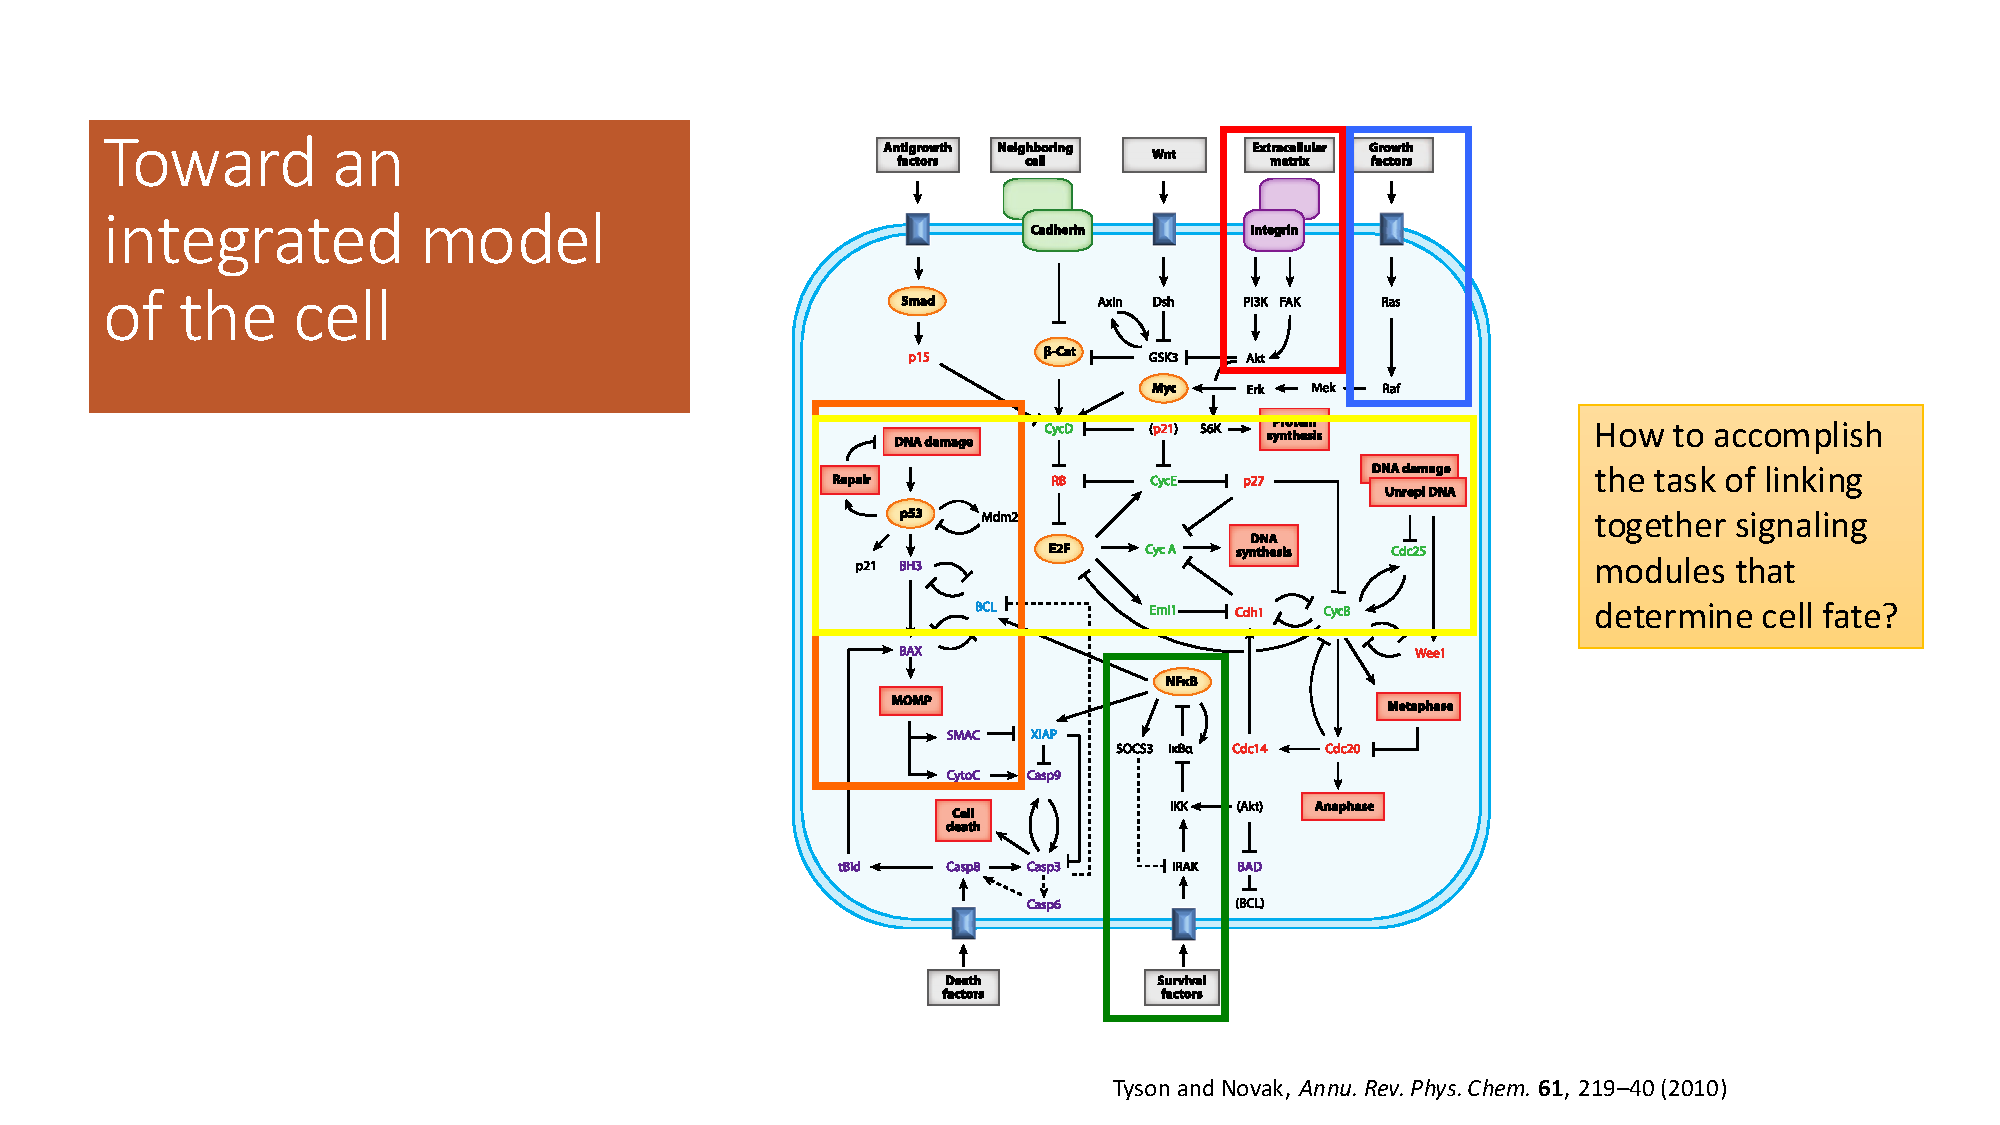
\includegraphics[height=0.7\textheight,trim=375 46 223 55,clip]{tyson_novak_2010.pdf}
    \end{column}
    \begin{column}{0.35\textwidth}
      Cell fate is decided by many interacting signaling modules: growth-factor
      signaling, the cell cycle, DNA damage, apoptosis.
      \vskip3mm
      \onslide<2->
      \hl{How do we link these modules together} into models that predict how
      cells respond?
    \end{column}
  \end{columns}
  \source{Tyson and Novak, \emph{Annu.\ Rev.\ Phys.\ Chem.}\ \textbf{61}, 219--240 (2010)}
\end{frame}

\begin{frame}{Large models are built from simple reaction steps}
  \centering
  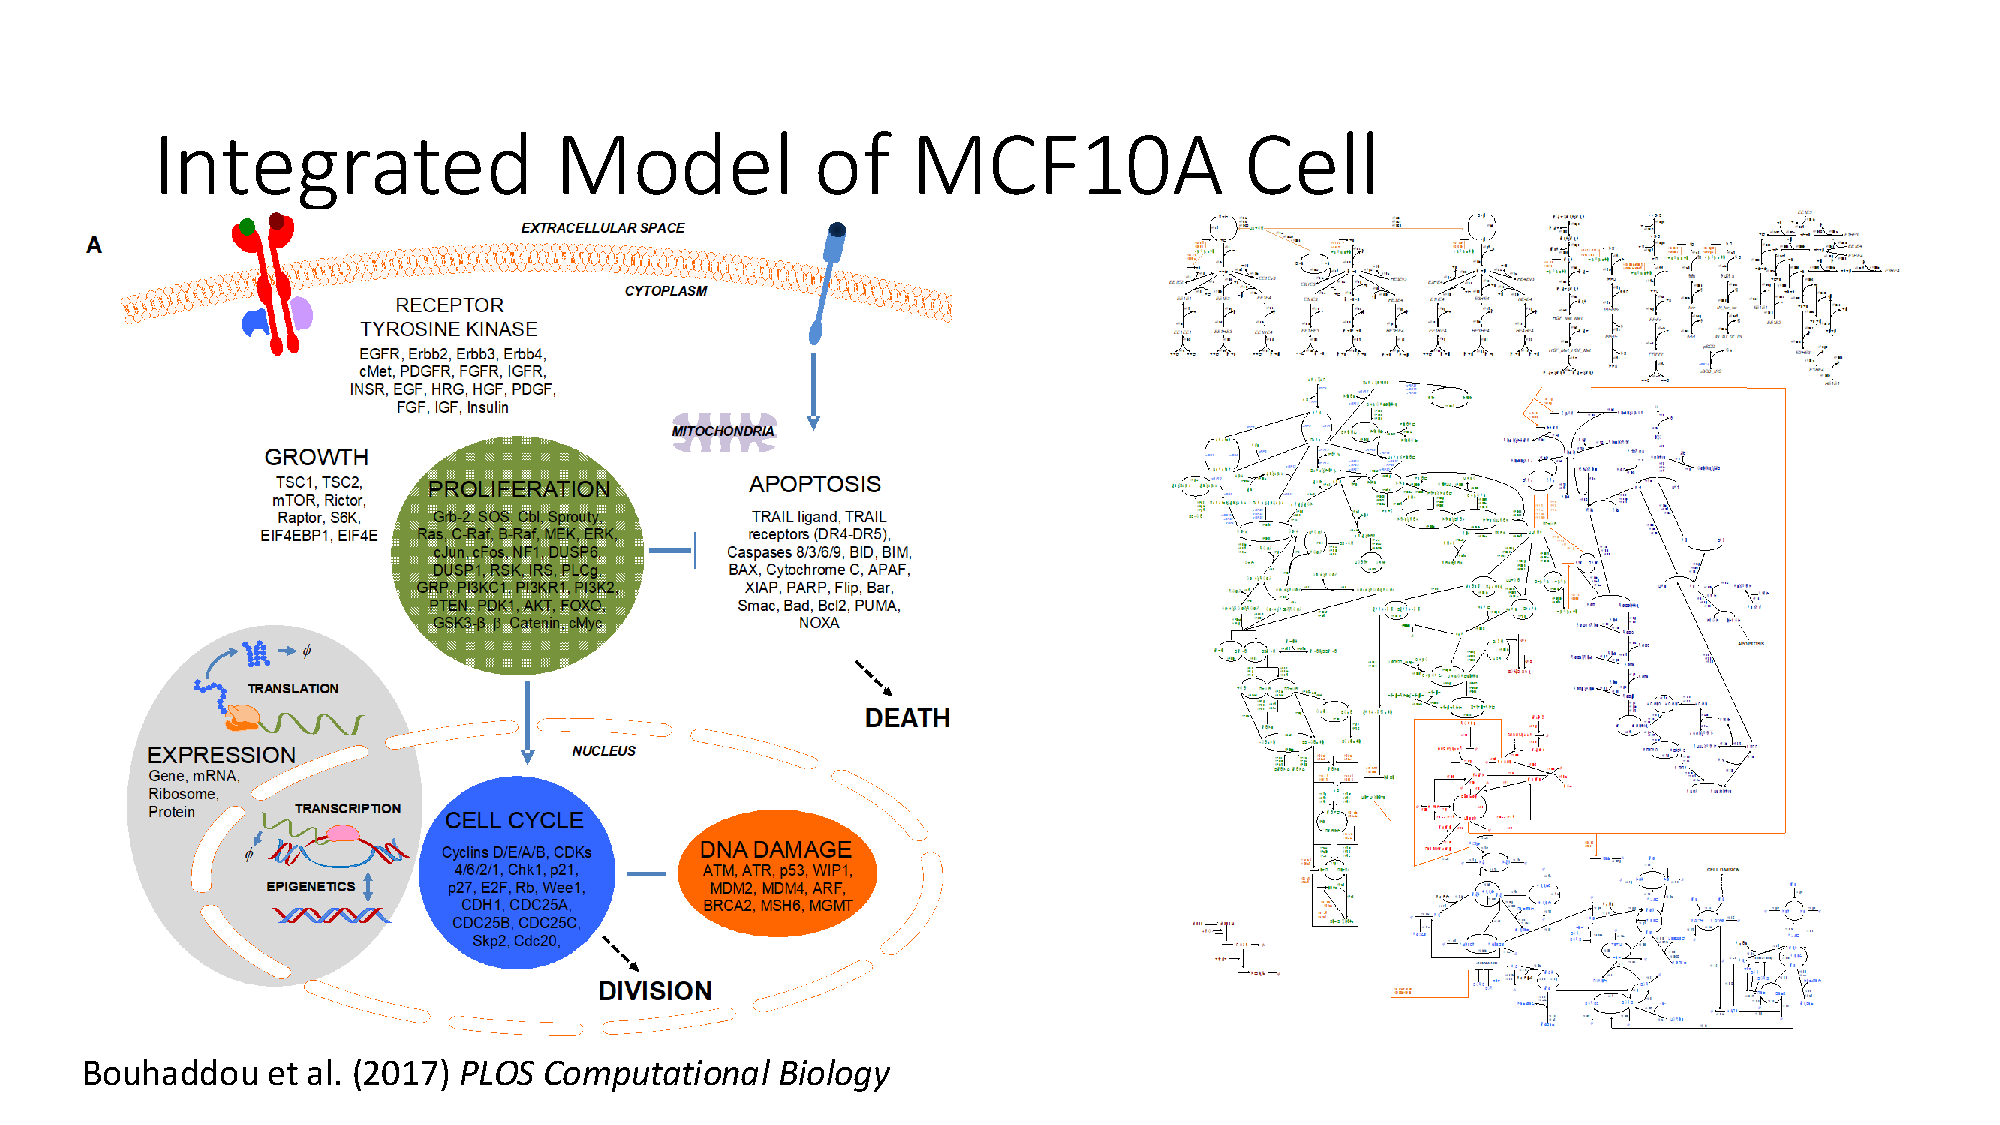
\includegraphics[width=0.94\textwidth,trim=38 40 47 100,clip]{bouhaddou_2018.pdf}
  \source{Bouhaddou et al., \emph{PLOS Comput.\ Biol.}\ (2018). Integrated model of an MCF10A cell.}
\end{frame}

% ======================================================================
\section{A cytokine signaling circuit}

\begin{frame}{Cytokines signal through receptors, STATs, and SOCS feedback}
  \begin{columns}[c]
    \begin{column}{0.45\textwidth}
      \small
      \begin{itemize}[<+->]
        \setlength\itemsep{1mm}
        \item \textbf{Cytokines} (e.g.\ interleukins, interferons) are secreted
              proteins that coordinate immune responses.
        \item Binding to their \textbf{receptor} activates receptor-associated
              JAK kinases.
        \item \textbf{STAT} transcription factors dock on the active receptor, are
              phosphorylated, and move to the nucleus.
        \item pSTAT induces genes including \textbf{SOCS} (suppressor of cytokine
              signaling).
        \item SOCS binds the receptor and \hl{shuts off further STAT activation}:
              negative feedback.
      \end{itemize}
    \end{column}
    \begin{column}{0.53\textwidth}
      \centering
      \only<1-2| handout:0>{\roadmap[scale=0.95]{1}}%
      \only<3| handout:0>{\roadmap[scale=0.95]{4}}%
      \only<4| handout:0>{\roadmap[scale=0.95]{5}}%
      \only<5-| handout:1>{\roadmap[scale=0.95]{99}}%
    \end{column}
  \end{columns}
\end{frame}

\begin{frame}{We will build the model one reaction step at a time}
  \begin{columns}[c]
    \begin{column}{0.45\textwidth}
      \begin{enumerate}[<+->]
        \setlength\itemsep{1.2mm}
        \item Ligand--receptor binding
        \item STAT binds the ligand-bound receptor
        \item Receptor-bound STAT is activated
        \item Activated STAT dissociates
        \item pSTAT binds the SOCS promoter;\\ SOCS is transcribed and translated
        \item SOCS binds the receptor and blocks STAT binding
      \end{enumerate}
      \vskip2mm
      \onslide<7->
      {\small Each step adds reactions to the previous model. The files are
      \code{models/stat\_step1\_binding.bngl} through
      \code{stat\_step6\_feedback.bngl}.}
    \end{column}
    \begin{column}{0.53\textwidth}
      \centering
      \only<1| handout:0>{\roadmap[scale=0.95]{1}}%
      \only<2| handout:0>{\roadmap[scale=0.95]{2}}%
      \only<3| handout:0>{\roadmap[scale=0.95]{3}}%
      \only<4| handout:0>{\roadmap[scale=0.95]{4}}%
      \only<5| handout:0>{\roadmap[scale=0.95]{5}}%
      \only<6| handout:0>{\roadmap[scale=0.95]{6}}%
      \only<7-| handout:1>{\roadmap[scale=0.95]{99}}%
    \end{column}
  \end{columns}
\end{frame}

% ======================================================================
\section{Step 1: Ligand--receptor binding}

\begin{frame}{Binding is a reversible pair of reactions}
  \begin{columns}[c]
    \begin{column}{0.55\textwidth}
      \[
        \mathsf{L} + \mathsf{R}
        \;\underset{k_\mathsf{off}}{\overset{k_\mathsf{on}}{\rightleftharpoons}}\;
        \mathsf{LR}
      \]
      \vskip1mm
      \onslide<2->
      Two elementary reactions, each with its own rate:
      \begin{align*}
        \text{binding:}   &\quad v_1 = k_\mathsf{on}\,\conc{L}\,\conc{R} \\
        \text{unbinding:} &\quad v_2 = k_\mathsf{off}\,\conc{LR}
      \end{align*}
      \onslide<3->
      \begin{block}{Law of mass action}
        \small The rate of an elementary reaction is proportional to the product of
        the concentrations of its reactants. The proportionality constant is the
        \textbf{rate constant}.
      \end{block}
    \end{column}
    \begin{column}{0.42\textwidth}
      \centering
      \onslide<1->
      \roadmap[scale=0.62]{1}
      \vskip2mm
      {\scriptsize Units: $k_\mathsf{on}$ in $\mu$M$^{-1}$min$^{-1}$,
      $k_\mathsf{off}$ in min$^{-1}$}
    \end{column}
  \end{columns}
\end{frame}

\begin{frame}{Each reaction contributes to the rate of change of its species}
  \begin{columns}[c]
    \begin{column}{0.5\textwidth}
      \centering
      \begin{tabular}{lcc}
        \toprule
        & $v_1$ (bind) & $v_2$ (unbind) \\
        \midrule
        L  & $-1$ & $+1$ \\
        R  & $-1$ & $+1$ \\
        LR & $+1$ & $-1$ \\
        \bottomrule
      \end{tabular}
      \vskip3mm
      {\small Reactants are consumed ($-$), products are created ($+$).}
    \end{column}
    \begin{column}{0.48\textwidth}
      \onslide<2->
      \begin{align*}
        \frac{d\conc{L}}{dt}  &= -k_\mathsf{on}\conc{L}\conc{R} + k_\mathsf{off}\conc{LR}\\[1mm]
        \frac{d\conc{R}}{dt}  &= -k_\mathsf{on}\conc{L}\conc{R} + k_\mathsf{off}\conc{LR}\\[1mm]
        \frac{d\conc{LR}}{dt} &= +k_\mathsf{on}\conc{L}\conc{R} - k_\mathsf{off}\conc{LR}
      \end{align*}
    \end{column}
  \end{columns}
  \onslide<3->
  \takeaway{Ordinary differential equations (ODEs) follow mechanically from the
  list of reactions and their rate laws.}
\end{frame}

\begin{frame}{The stoichiometry matrix gives a compact general form}
  Collect the concentrations in a vector $\mathbf{X}$ and the reaction rates in $\mathbf{v}$:
  \[
    \frac{d\mathbf{X}}{dt} = \mathbf{S}\,\mathbf{v}(\mathbf{X}),
    \qquad
    \frac{d}{dt}\begin{pmatrix}\conc{L}\\ \conc{R}\\ \conc{LR}\end{pmatrix}
    =
    \underbrace{\begin{pmatrix}-1 & +1\\ -1 & +1\\ +1 & -1\end{pmatrix}}_{\mathbf{S}}
    \underbrace{\begin{pmatrix}k_\mathsf{on}\conc{L}\conc{R}\\ k_\mathsf{off}\conc{LR}\end{pmatrix}}_{\mathbf{v}(\mathbf{X})}
  \]
  \vskip1mm
  \onslide<2->
  \[
    S_{ij} = (\text{times species } i \text{ is a product of reaction } j)
           - (\text{times species } i \text{ is a reactant of reaction } j)
  \]
  \begin{itemize}
    \item<3-> $\mathbf{S}$ has one row per species and one column per reaction.
    \item<4-> This form holds for \emph{any} reaction network; only $\mathbf{S}$ and
          $\mathbf{v}$ change.
  \end{itemize}
\end{frame}

\begin{frame}{Conservation laws and equilibrium}
  \begin{columns}[T]
    \begin{column}{0.5\textwidth}
      \textbf{Conservation.} Binding only moves molecules between free and bound forms:
      \begin{align*}
        \conc{L} + \conc{LR} &= L_0\\
        \conc{R} + \conc{LR} &= R_0
      \end{align*}
      so only one of the three ODEs is independent.
      \vskip2mm
      {\small These appear as linear dependencies among the rows of $\mathbf{S}$.}
    \end{column}
    \begin{column}{0.48\textwidth}
      \onslide<2->
      \textbf{Equilibrium.} At steady state $v_1 = v_2$:
      \[
        \frac{\conc{L}\conc{R}}{\conc{LR}} = \frac{k_\mathsf{off}}{k_\mathsf{on}} \equiv K_D
      \]
      \onslide<3->
      Substituting the conservation laws gives a quadratic for $\conc{LR}$:
      \[
        \conc{LR}_\mathsf{eq} = \tfrac12\!\left[\,b - \sqrt{b^2 - 4L_0R_0}\,\right],
      \]
      \[
        b = L_0 + R_0 + K_D
      \]
    \end{column}
  \end{columns}
  \onslide<4->
  \takeaway{Small models can be solved by hand. Real signaling networks cannot,
  so we solve the ODEs numerically.}
\end{frame}

\begin{frame}{ODEs for reaction networks are solved numerically}
  \begin{columns}[T]
    \begin{column}{0.55\textwidth}
      Simplest idea (forward Euler): take small time steps $\Delta t$,
      \[
        \mathbf{X}(t+\Delta t) \approx \mathbf{X}(t) + \Delta t\;\mathbf{S}\,\mathbf{v}(\mathbf{X}(t))
      \]
      \onslide<2->
      In practice:
      \begin{itemize}
        \item<2-> The equations are \textbf{nonlinear} and usually have no closed-form solution.
        \item<3-> Reactions occur on very different time scales, which makes the system
              \textbf{stiff}: simple methods need impractically small steps.
        \item<4-> Production solvers (CVODE, LSODA) adapt the step size and use implicit
              methods for stiff systems.
      \end{itemize}
    \end{column}
    \begin{column}{0.42\textwidth}
      \onslide<5->
      \begin{block}{In BioNetGen}
        \small
        \code{simulate(\{method=>"ode",...\})} \\
        uses CVODE.
        \vskip1mm
        In Python, \code{model.setup\_simulator()} returns a libRoadRunner simulator
        for the same model.
      \end{block}
    \end{column}
  \end{columns}
\end{frame}

\begin{frame}{Binding approaches equilibrium faster and further at higher ligand}
  \begin{columns}[c]
    \begin{column}{0.58\textwidth}
      \begin{tikzpicture}
        \begin{axis}[fsplot, ylabel={$\conc{LR}$ ($\mu$M)}, xmax=2, ymax=1.1,
                     legend style={at={(0.98,0.16)},anchor=south east}]
          \addplot table[x=time,y=LR]{data/lr_dose_L10.dat};  \addlegendentry{$L_0=10$}
          \addplot table[x=time,y=LR]{data/lr_dose_L1.dat};   \addlegendentry{$L_0=1$}
          \addplot table[x=time,y=LR]{data/lr_dose_L0.1.dat}; \addlegendentry{$L_0=0.1$}
          \addplot[fsNavy,dashed,line width=0.6pt,domain=0:2,visible on=<2->]{0.9892};
          \addplot[fsAccent,dashed,line width=0.6pt,domain=0:2,visible on=<2->]{0.7298};
          \addplot[fsTeal,dashed,line width=0.6pt,domain=0:2,visible on=<2->]{0.0901};
        \end{axis}
      \end{tikzpicture}
    \end{column}
    \begin{column}{0.4\textwidth}
      \small
      $R_0 = 1\,\mu$M, $k_\mathsf{on} = 1\,\mu$M$^{-1}$min$^{-1}$,
      $k_\mathsf{off} = 0.1\,$min$^{-1}$ ($K_D = 0.1\,\mu$M).
      \vskip2mm
      \onslide<2->
      Dashed lines: $\conc{LR}_\mathsf{eq}$ from the formula on the previous slide.
      \vskip2mm
      \onslide<3->
      The relaxation rate is $k_\mathsf{on}(\conc{L}+\conc{R}) + k_\mathsf{off}$
      near equilibrium, so higher ligand also means a faster response.
    \end{column}
  \end{columns}
\end{frame}

\begin{frame}[fragile]{The same model in BNGL}
  \begin{columns}[T]
    \begin{column}{0.49\textwidth}
      \lstinputlisting[language=bngl,firstline=6,lastline=24,basicstyle=\ttfamily\scriptsize]{\modeldir/stat_step1_binding.bngl}
    \end{column}
    \begin{column}{0.49\textwidth}
      \onslide<2->
      \lstinputlisting[language=bngl,firstline=26,lastline=40,basicstyle=\ttfamily\scriptsize]{\modeldir/stat_step1_binding.bngl}
      \vskip1mm
      {\scriptsize
      \begin{itemize}
        \item<3-> \textbf{observables}: quantities to output
        \item<4-> \textbf{reaction rules}: \code{<->} is reversible; forward and reverse rate constants
        \item<5-> \textbf{actions} after \code{end model}: generate the network, then simulate
      \end{itemize}}
    \end{column}
  \end{columns}
\end{frame}

\begin{frame}{Running a model in VS Code}
  \begin{columns}[c]
    \begin{column}{0.68\textwidth}
      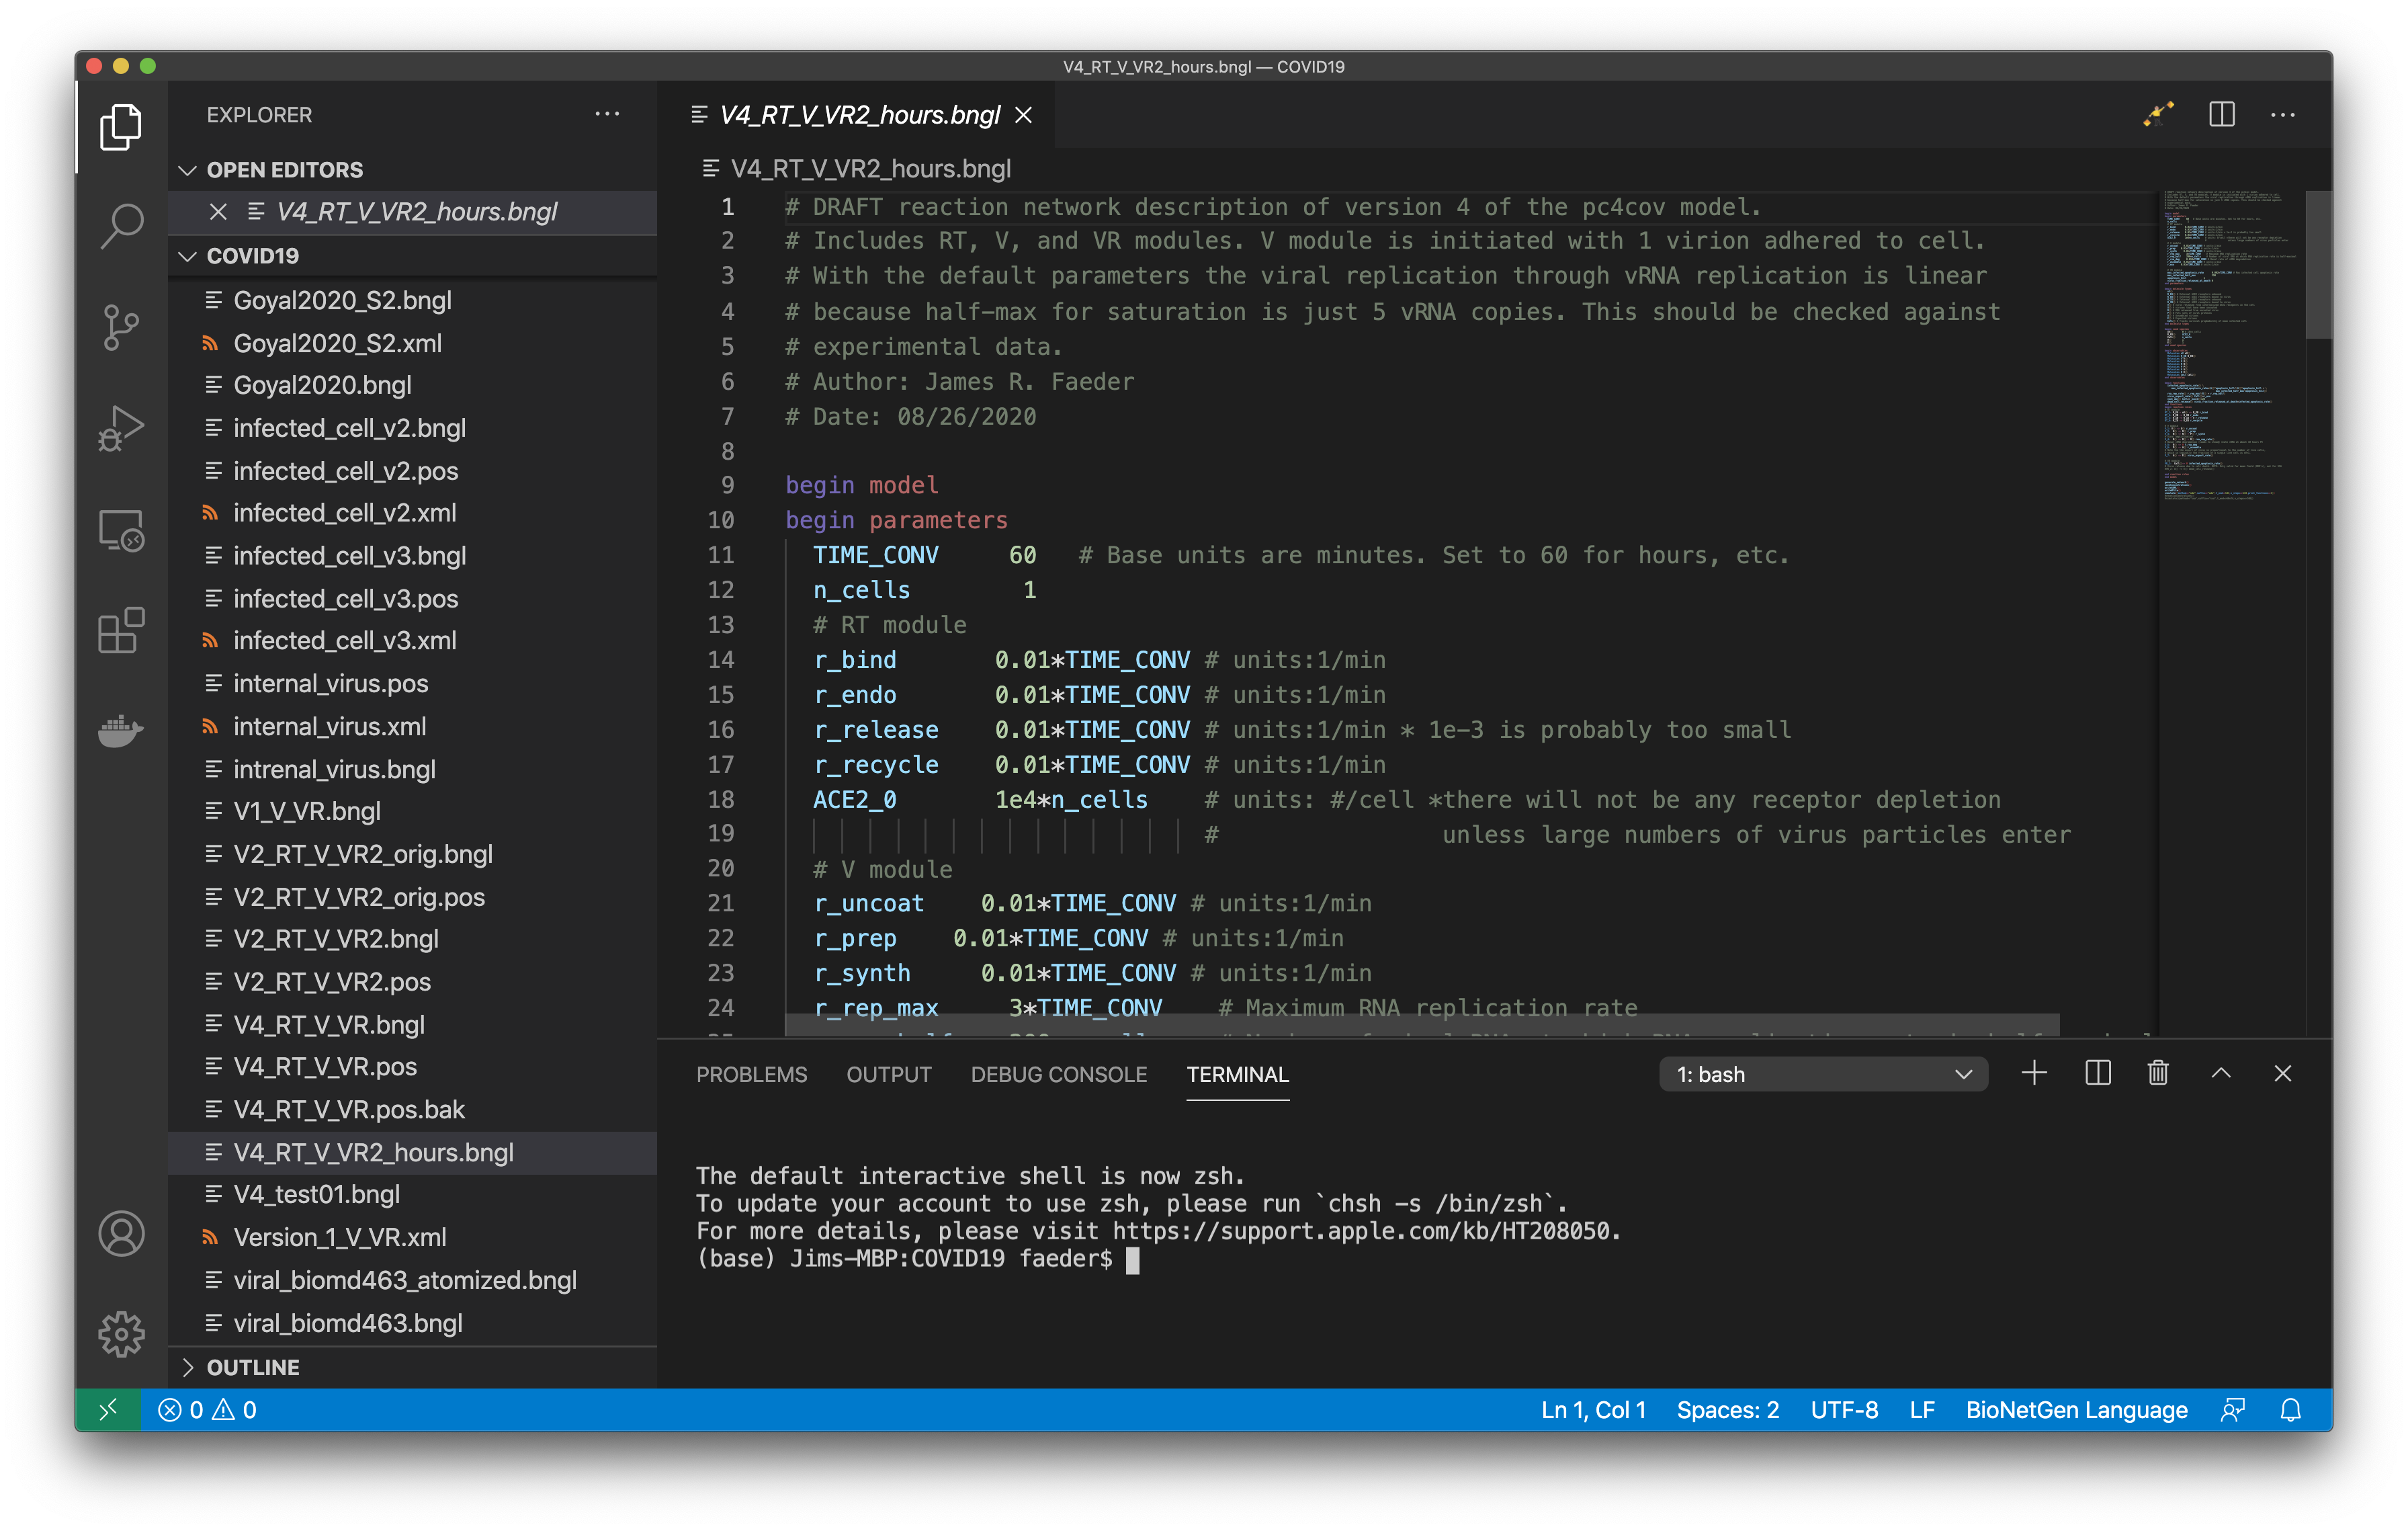
\includegraphics[width=0.92\linewidth]{vscode_run.png}
    \end{column}
    \begin{column}{0.3\textwidth}
      \small
      \begin{itemize}[<+->]
        \item Open a \code{.bngl} file
        \item Click the \hl{run} button in the editor toolbar
        \item Results go to\\ \code{BNG-results/<model>/}\\ \code{\ \ <timestamp>/}
      \end{itemize}
    \end{column}
  \end{columns}
  \source{VS Code extension: Ali Sinan Saglam}
\end{frame}

\begin{frame}{Interactive plotting and Python notebooks}
  \begin{columns}[T]
    \begin{column}{0.49\textwidth}
      \centering
      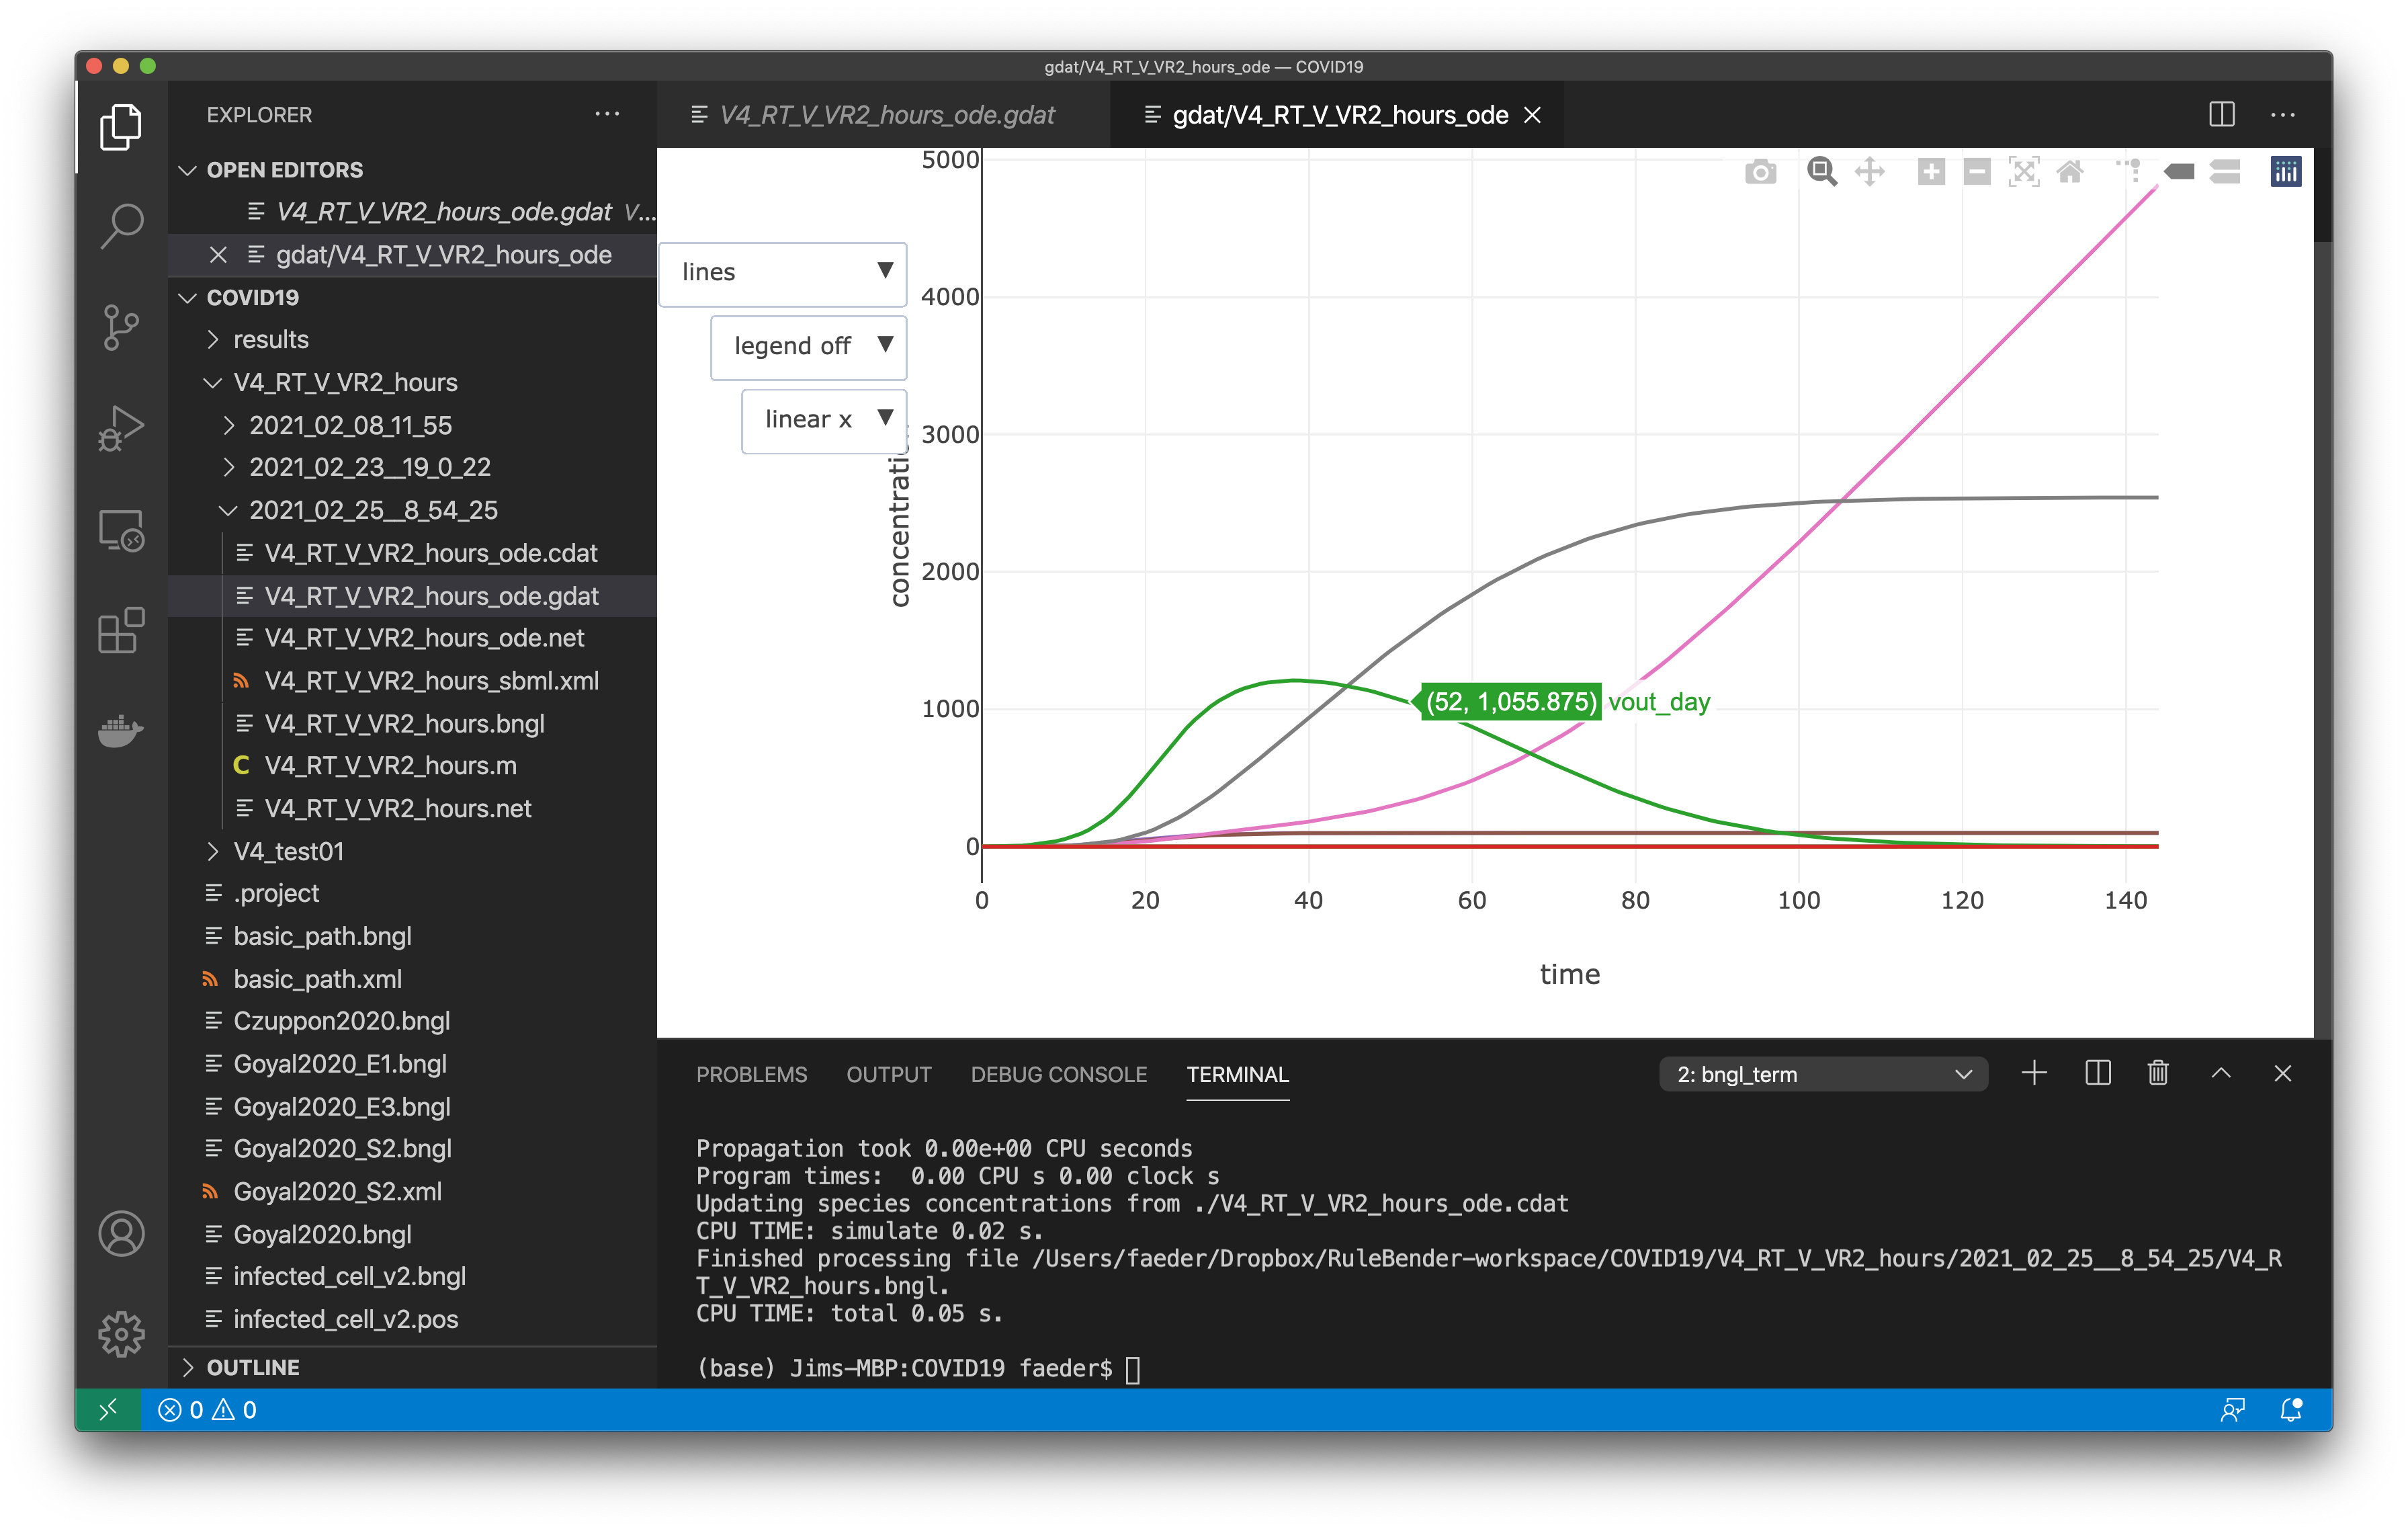
\includegraphics[width=\linewidth]{vscode_plot.png}\\[1mm]
      {\small Built-in plotting of \code{.gdat} output}
    \end{column}
    \begin{column}{0.49\textwidth}
      \centering
      \onslide<2->
      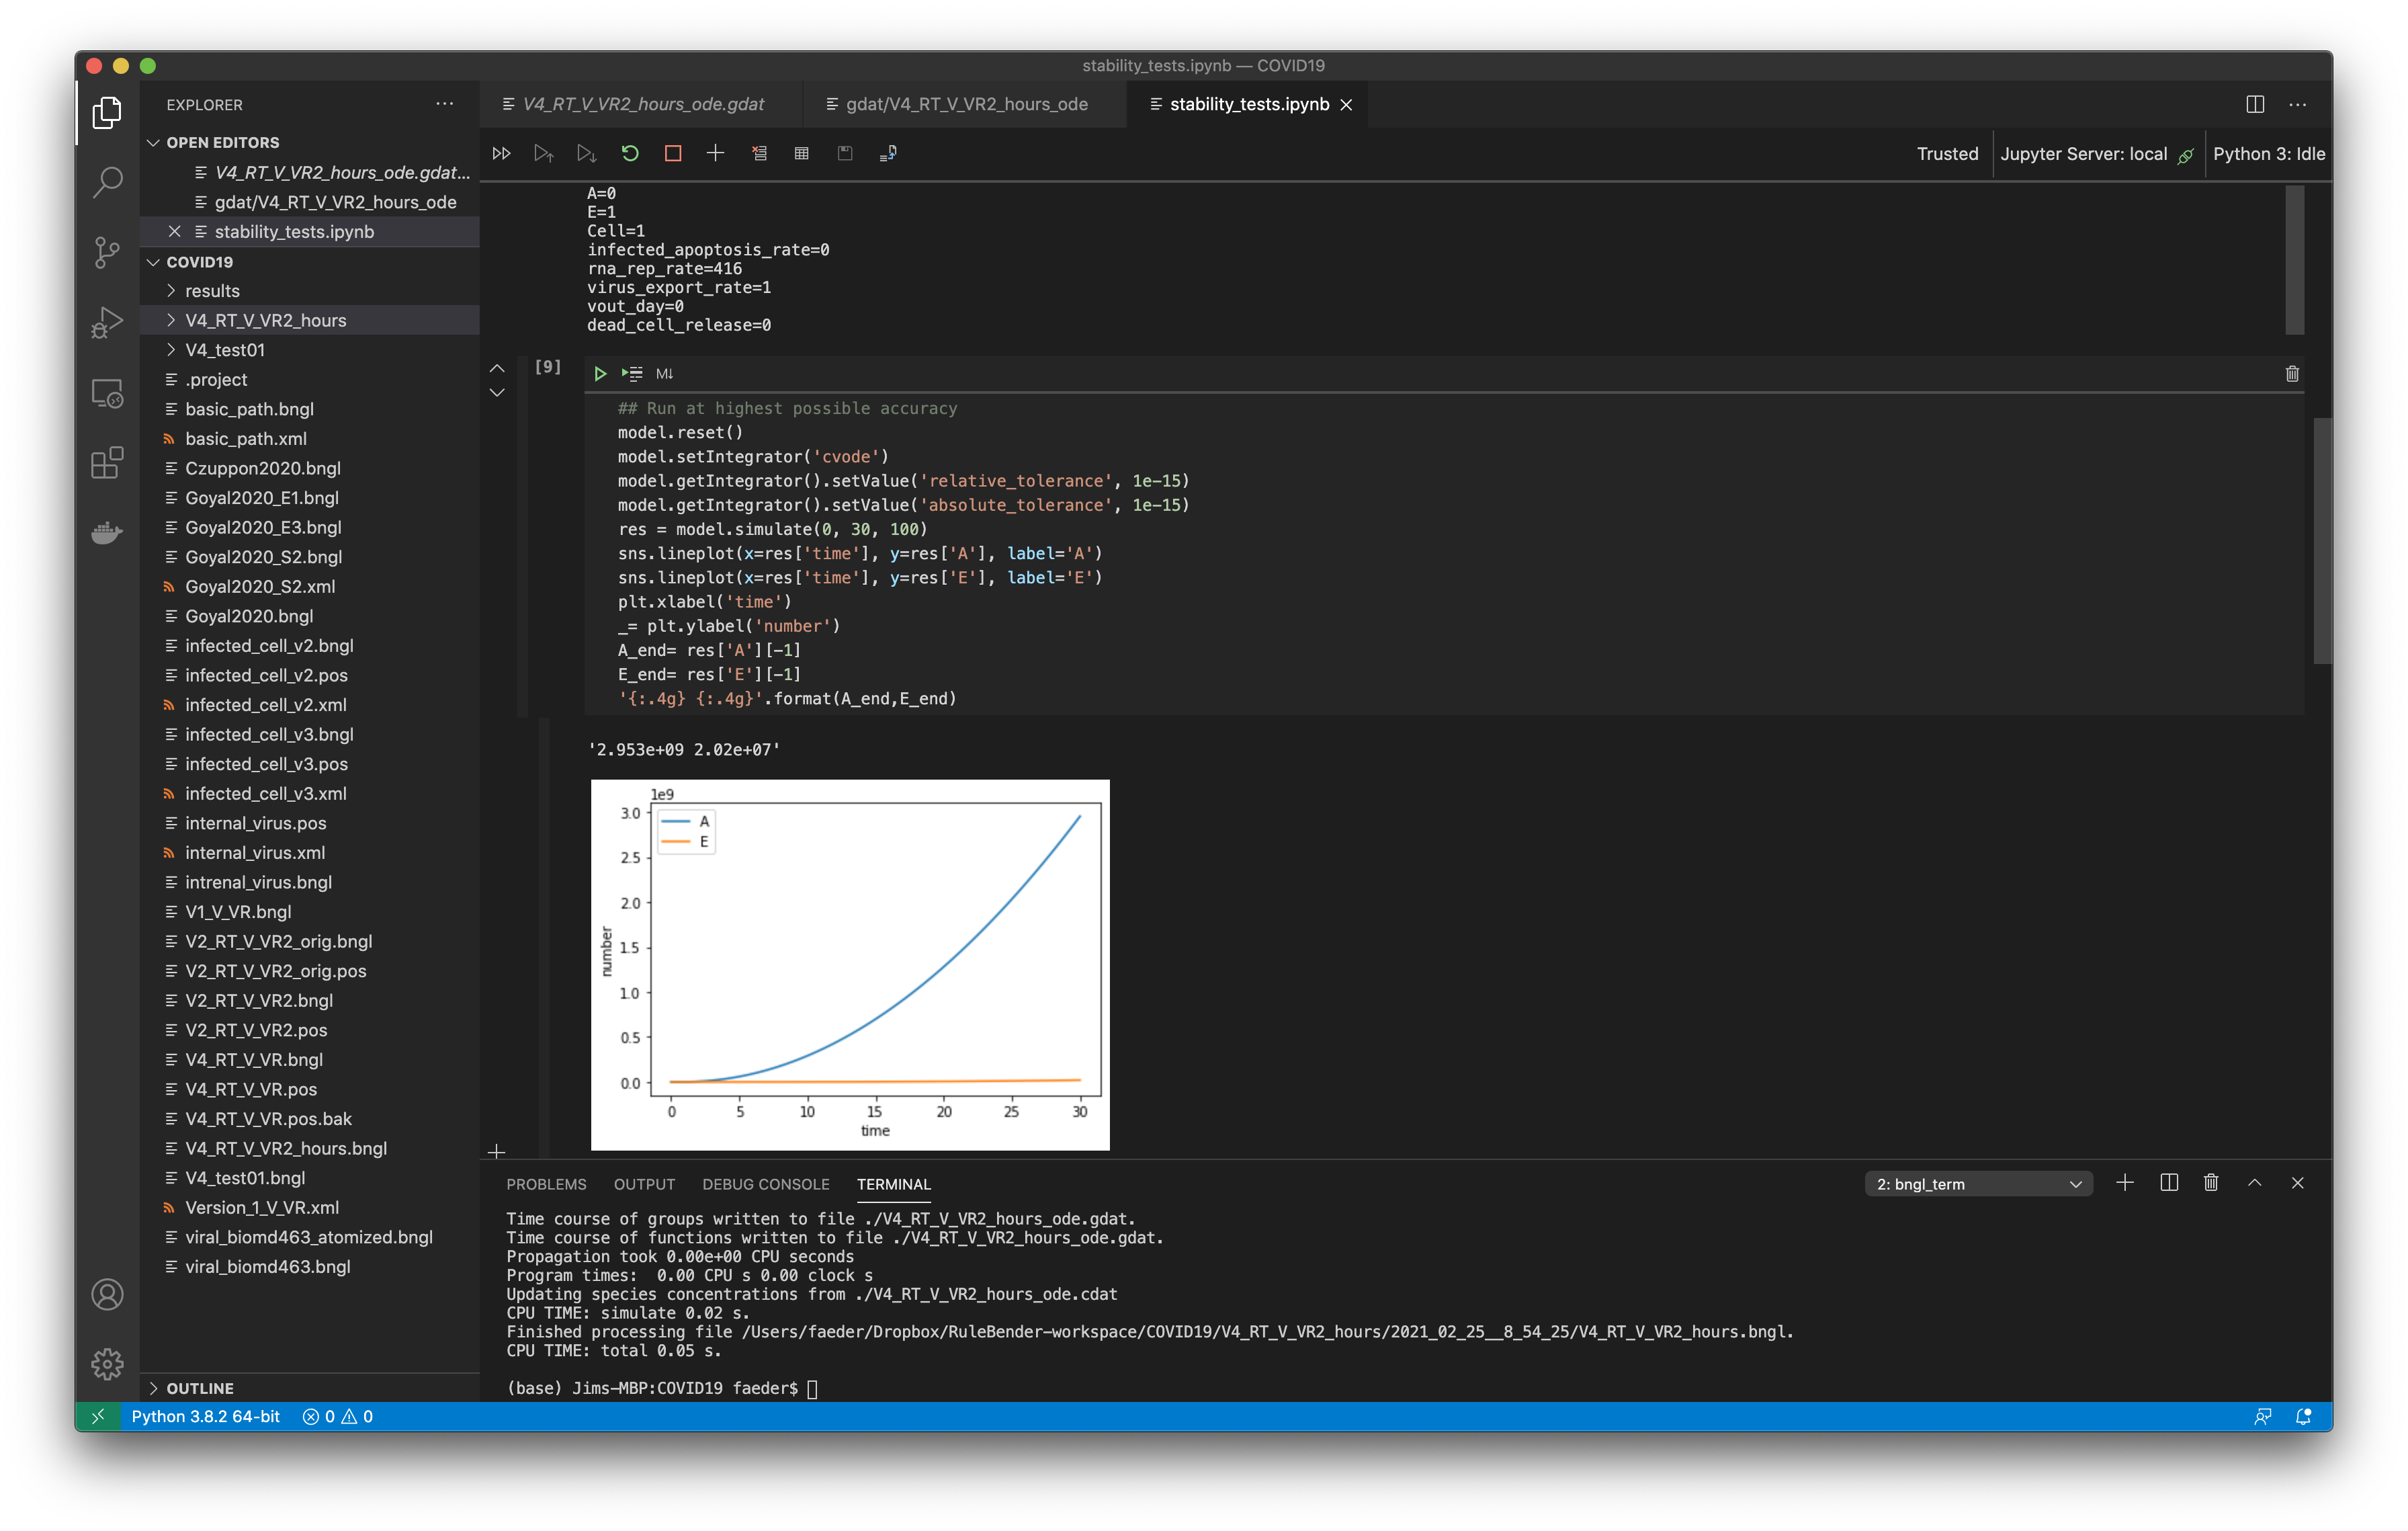
\includegraphics[width=\linewidth]{vscode_notebook.png}\\[1mm]
      {\small Deeper analysis in Jupyter with PyBioNetGen + libRoadRunner}
    \end{column}
  \end{columns}
\end{frame}

\begin{frame}{BNG Playground: BioNetGen in your browser}
  \begin{columns}[c]
    \begin{column}{0.6\textwidth}
      \begin{itemize}[<+->]
        \setlength\itemsep{2mm}
        \item Write, simulate, and analyze BNGL models in a web browser:
              nothing to install
        \item Interactive examples for learning rule-based modeling
        \item Share a model as a link
        \item Useful for trying the course models on any computer:
              paste a file from \code{models/} and run it
      \end{itemize}
    \end{column}
    \begin{column}{0.36\textwidth}
      \centering
      \qrcode[height=3.6cm]{\bngplayground}\\[2mm]
      \href{\bngplayground}{\small ruleworld.github.io/bngplayground}
    \end{column}
  \end{columns}
\end{frame}

% ======================================================================
\section{Building the signaling circuit in BNGL}

\begin{frame}[fragile]{Step 2: STAT binds the ligand-bound receptor}
  \begin{columns}[T]
    \begin{column}{0.5\textwidth}
      \[
        \mathsf{LR} + \mathsf{S} \rightleftharpoons \mathsf{LRS}
      \]
      \onslide<3->
      New lines in \code{stat\_step2\_recruit.bngl}:
\begin{lstlisting}[language=bngl,basicstyle=\ttfamily\scriptsize]
begin parameters
  S0     10   # STAT (uM)
  kSon   1    # STAT binding (1/uM/min)
  kSoff  1    # STAT unbinding (1/min)
end parameters
begin molecule types
  S
  LRS
end molecule types
begin species
  S  S0
end species
begin reaction rules
  Sbind: LR + S <-> LRS kSon, kSoff
end reaction rules
\end{lstlisting}
    \end{column}
    \begin{column}{0.46\textwidth}
      \centering
      \onslide<1->
      \roadmap[scale=0.55]{2}
      \vskip2mm
      \raggedright
      \onslide<2->
      STAT can bind \emph{only} the ligand-bound receptor LR, never free R.
      This is how ligand binding \hl{enables} STAT recruitment.
      \vskip2mm
      \onslide<4->
      {\small Every new species needs a molecule type; species present at $t=0$
      also need an initial amount.}
    \end{column}
  \end{columns}
\end{frame}

\begin{frame}[fragile]{Step 3: receptor-bound STAT is activated}
  \begin{columns}[T]
    \begin{column}{0.5\textwidth}
      \[
        \mathsf{LRS} \xrightarrow{\;k_\mathsf{act}\;} \mathsf{LRS_p}
      \]
      A receptor-associated kinase (JAK) phosphorylates the docked STAT:
      a \textbf{first-order}, irreversible reaction with $v = k_\mathsf{act}\conc{LRS}$.
      \onslide<2->
\begin{lstlisting}[language=bngl]
  kact  1   # STAT activation (1/min)
  LRSp
  Sact: LRS -> LRSp kact
\end{lstlisting}
      {\scriptsize\color{fsGray}one new line each in parameters, molecule types, and reaction rules}
      \vskip3mm
      \onslide<4->
      \hl{Problem:} pSTAT never leaves the receptor. Every receptor ends up
      stuck as LRS$_\mathsf{p}$.
    \end{column}
    \begin{column}{0.46\textwidth}
      \centering
      \onslide<1->
      \roadmap[scale=0.42]{3}\\[1mm]
      \onslide<3->
      \begin{tikzpicture}
        \begin{axis}[fsplot,width=0.95\linewidth,height=0.5\linewidth,ylabel={$\mu$M},xmax=15,legend above]
          \addplot table[x=time,y=LR]{data/stat_step3_activate.dat};   \addlegendentry{LR}
          \addplot table[x=time,y=LRS]{data/stat_step3_activate.dat};  \addlegendentry{LRS}
          \addplot table[x=time,y=LRSp]{data/stat_step3_activate.dat}; \addlegendentry{LRS$_\mathsf{p}$}
        \end{axis}
      \end{tikzpicture}
    \end{column}
  \end{columns}
\end{frame}

\begin{frame}[fragile]{Step 4: activated STAT dissociates from the receptor}
  \begin{columns}[T]
    \begin{column}{0.5\textwidth}
      \[
        \mathsf{LRS_p} \xrightarrow{\;k_\mathsf{diss}\;} \mathsf{LR} + \mathsf{S_p}
        \qquad
        \mathsf{S_p} \xrightarrow{\;k_\mathsf{dephos}\;} \mathsf{S}
      \]
      Releasing pSTAT frees the receptor to activate another STAT.
      A phosphatase returns free pSTAT to the inactive pool.
      \onslide<2->
\begin{lstlisting}[language=bngl]
  kdiss    1    # pSTAT release (1/min)
  kdephos  0.1  # dephosphorylation (1/min)
  Sp
  Srelease: LRSp -> LR + Sp kdiss
  Sdephos:  Sp -> S kdephos
\end{lstlisting}
      \onslide<4->
      pSTAT now reaches a steady state set by the balance of activation and
      dephosphorylation.
    \end{column}
    \begin{column}{0.46\textwidth}
      \centering
      \onslide<1->
      \roadmap[scale=0.42]{4}\\[1mm]
      \onslide<3->
      \begin{tikzpicture}
        \begin{axis}[fsplot,width=0.95\linewidth,height=0.5\linewidth,ylabel={$\mu$M},legend above]
          \addplot table[x=time,y=pSTAT]{data/stat_step4_release.dat}; \addlegendentry{total pSTAT}
          \addplot table[x=time,y=Sfree]{data/stat_step4_release.dat}; \addlegendentry{inactive STAT}
        \end{axis}
      \end{tikzpicture}
    \end{column}
  \end{columns}
\end{frame}

\begin{frame}[fragile]{Step 5: pSTAT induces SOCS expression}
  \begin{columns}[T]
    \begin{column}{0.52\textwidth}
\begin{lstlisting}[language=bngl,basicstyle=\ttfamily\scriptsize]
  # pSTAT binds the SOCS promoter
  Gbind: Sp + G <-> GSp kGon, kGoff
  # Bound promoter is transcribed
  Transcribe: GSp -> GSp + mSOCS ktx
  # mRNA degradation
  mRNAdeg: mSOCS -> 0 kmdeg
  # Translation
  Translate: mSOCS -> mSOCS + SOCS ktl
  # SOCS protein degradation
  SOCSdeg: SOCS -> 0 kSOCSdeg
\end{lstlisting}
      \small
      \begin{itemize}
        \item<2-> \textbf{Synthesis}: a species on both sides (\code{GSp}, \code{mSOCS})
              is a template and is not consumed.
        \item<3-> \textbf{Degradation}: \code{0} means nothing; the molecule is removed.
      \end{itemize}
      \vskip1mm
      \onslide<5->
      SOCS accumulates, but it has no target yet, so pSTAT is unaffected.
    \end{column}
    \begin{column}{0.44\textwidth}
      \centering
      \onslide<1->
      \roadmap[scale=0.42]{5}\\[1mm]
      \onslide<4->
      \begin{tikzpicture}
        \begin{axis}[fsplot,width=0.95\linewidth,height=0.5\linewidth,ylabel={$\mu$M},legend above]
          \addplot table[x=time,y=pSTAT]{data/stat_step5_transcribe.dat}; \addlegendentry{pSTAT}
          \addplot table[x=time,y=mSOCS]{data/stat_step5_transcribe.dat}; \addlegendentry{SOCS mRNA}
          \addplot table[x=time,y=SOCS]{data/stat_step5_transcribe.dat};  \addlegendentry{SOCS}
        \end{axis}
      \end{tikzpicture}
    \end{column}
  \end{columns}
\end{frame}

\begin{frame}[fragile]{Step 6: SOCS binds the receptor and blocks STAT recruitment}
  \begin{columns}[c]
    \begin{column}{0.54\textwidth}
      \[
        \mathsf{LR} + \mathsf{SOCS} \rightleftharpoons \mathsf{LR{\cdot}SOCS}
      \]
      SOCS competes with STAT for the active receptor. LR$\cdot$SOCS cannot recruit STAT,
      so pSTAT production drops.
      \onslide<2->
      The loop is closed:
      \[
        \text{pSTAT} \to \text{SOCS} \dashv \text{receptor} \to \text{pSTAT}
      \]
      \onslide<3->
\begin{lstlisting}[language=bngl]
  kSOCSon   1     # (1/uM/min)
  kSOCSoff  0.01  # (1/min)
  LRSOCS
  SOCSbind: LR + SOCS <-> LRSOCS kSOCSon, kSOCSoff
\end{lstlisting}
    \end{column}
    \begin{column}{0.44\textwidth}
      \centering
      \onslide<1->
      \roadmap[scale=0.62]{6}
    \end{column}
  \end{columns}
\end{frame}

\begin{frame}{Negative feedback turns a sustained signal into a pulse}
  \begin{columns}[c]
    \begin{column}{0.6\textwidth}
      \begin{tikzpicture}
        \begin{axis}[fsplot, ylabel={total pSTAT ($\mu$M)}, xmax=120, ymax=6,
                     legend style={at={(0.98,0.22)},anchor=south east}]
          \addplot table[x=time,y=pSTAT]{data/stat_step6_no_feedback.dat}; \addlegendentry{without feedback (\code{kSOCSon = 0})}
          \only<2->{\addplot table[x=time,y=pSTAT]{data/stat_step6_feedback.dat};    \addlegendentry{with SOCS feedback}}
        \end{axis}
      \end{tikzpicture}
    \end{column}
    \begin{column}{0.38\textwidth}
      \small
      \begin{itemize}
        \setlength\itemsep{1.5mm}
        \item<3-> Early response is identical: SOCS has not been made yet.
        \item<4-> As SOCS accumulates it sequesters receptors, and pSTAT falls to a low
              level despite continued ligand.
        \item<5-> The delay comes from transcription and translation.
      \end{itemize}
      \vskip2mm
      \onslide<5->
      {\scriptsize Both curves come from \code{stat\_step6\_feedback.bngl}, which runs
      the model twice using \code{setParameter}.}
    \end{column}
  \end{columns}
\end{frame}

\begin{frame}{The complete network}
  \begin{columns}[T]
    \begin{column}{0.5\textwidth}
      \small
      \begin{tabular}{@{}rll@{}}
        \toprule
        & reaction & rate \\
        \midrule
        1 & L + R $\rightleftharpoons$ LR & $k_\mathsf{on}, k_\mathsf{off}$\\
        2 & LR + S $\rightleftharpoons$ LRS & $k_\mathsf{Son}, k_\mathsf{Soff}$\\
        3 & LRS $\to$ LRS$_\mathsf{p}$ & $k_\mathsf{act}$\\
        4 & LRS$_\mathsf{p}$ $\to$ LR + S$_\mathsf{p}$ & $k_\mathsf{diss}$\\
          & S$_\mathsf{p}$ $\to$ S & $k_\mathsf{dephos}$\\
        5 & S$_\mathsf{p}$ + G $\rightleftharpoons$ GS$_\mathsf{p}$ & $k_\mathsf{Gon}, k_\mathsf{Goff}$\\
          & GS$_\mathsf{p}$ $\to$ GS$_\mathsf{p}$ + mSOCS & $k_\mathsf{tx}$\\
          & mSOCS $\to$ 0 & $k_\mathsf{mdeg}$\\
          & mSOCS $\to$ mSOCS + SOCS & $k_\mathsf{tl}$\\
          & SOCS $\to$ 0 & $k_\mathsf{SOCSdeg}$\\
        6 & LR + SOCS $\rightleftharpoons$ LR$\cdot$SOCS & $k_\mathsf{SOCSon}, k_\mathsf{SOCSoff}$\\
        \bottomrule
      \end{tabular}
    \end{column}
    \begin{column}{0.46\textwidth}
      \begin{itemize}[<+(1)->]
        \setlength\itemsep{1.5mm}
        \item 11 lines of BNGL generate \textbf{15 reactions} (4 are reversible)
              among \textbf{12 species}.
        \item $\mathbf{S}$ is a $12\times15$ matrix; BioNetGen builds it and the ODEs
              for you (see the \code{.net} file).
        \item Every species had to be named by hand: L, LR, LRS, LRS$_\mathsf{p}$,
              LR$\cdot$SOCS, \ldots
      \end{itemize}
    \end{column}
  \end{columns}
\end{frame}

% ======================================================================
\section{Looking ahead}

\begin{frame}{Naming every complex by hand does not scale}
  Our model made strong simplifying assumptions. Relax a few of them:
  \begin{itemize}[<+->]
    \item SOCS can also bind receptors that already carry STAT (LRS, LRS$_\mathsf{p}$)
    \item Ligand can dissociate from \emph{any} receptor complex, not only LR
    \item The receptor has two chains, each recruiting its own STAT
    \item STATs dimerize before entering the nucleus
  \end{itemize}
  \vskip2mm
  \onslide<+->
  Each feature \hl{multiplies} the number of distinct complexes, and each complex
  needs its own species name and its own copy of every reaction it takes part in.
  \onslide<+->
  \takeaway{Module 2: represent molecules with internal structure (binding sites and
  states) and write rules that generate the network automatically.}
\end{frame}

\begin{frame}{ODEs describe average behavior}
  \begin{itemize}[<+->]
    \item ODEs treat concentrations as continuous and deterministic.
    \item In a single cell, some species are present in very small numbers:
          one or two copies of a gene, a few mRNA molecules.
    \item Then random timing of individual reactions matters, and cells with identical
          parameters respond differently.
    \item The \textbf{same reaction network} can be simulated stochastically with the
          Gillespie algorithm: \code{simulate(\{method=>"ssa",...\})}.
  \end{itemize}
  \vskip2mm
  \onslide<+->
  {\color{fsGray} We return to stochastic simulation in a later module.}
\end{frame}

\begin{frame}{Try it yourself}
  Using the models in \code{models/}:
  \begin{enumerate}
    \setlength\itemsep{1.5mm}
    \item Run \code{stat\_step1\_binding.bngl} at several values of \code{L0} and check
          the equilibrium against the formula for $\conc{LR}_\mathsf{eq}$.
    \item In \code{stat\_step4\_release.bngl}, set \code{kdephos} to 0. What happens
          to pSTAT, and why?
    \item In \code{stat\_step6\_feedback.bngl}, vary \code{ktl} (translation rate).
          How do the peak and the late level of pSTAT change?
    \item Add a reaction that lets SOCS bind \code{LRS} as well as \code{LR}.
          What new species do you need?
  \end{enumerate}
  \vskip3mm
  {\small No local setup yet? Paste any of these models into
  \href{\bngplayground}{BNG Playground} (\code{ruleworld.github.io/bngplayground})
  and run it in your browser.}
\end{frame}

\begin{frame}{Summary}
  \begin{itemize}[<+->]
    \setlength\itemsep{2mm}
    \item A reaction network is defined by its species, reactions, rate laws, and
          initial conditions.
    \item Mass-action rate laws turn the network into ODEs:
          $d\mathbf{X}/dt = \mathbf{S}\,\mathbf{v}(\mathbf{X})$.
    \item BNGL describes the network directly; BioNetGen generates and integrates the ODEs.
    \item Building the cytokine--STAT--SOCS circuit one step at a time shows how each
          mechanism contributes; negative feedback produces an adaptive pulse of pSTAT.
    \item Writing every complex as a separate species quickly becomes unmanageable.
          This motivates rule-based modeling, the subject of Module 2.
  \end{itemize}
\end{frame}

\end{document}
